\documentclass[11pt,a4paper]{article}

\usepackage[utf8]{inputenc}
\usepackage[T1]{fontenc}
\usepackage[danish]{babel}
\usepackage{lmodern}
\usepackage[margin=2.5cm]{geometry}
\usepackage{graphicx}
\usepackage{booktabs}
\usepackage{subcaption}
\usepackage{microtype}
\usepackage[hidelinks]{hyperref}
\usepackage{parskip}

\graphicspath{{../exercise1_2/plots/}}

\title{Tegnbaserede sprogmodeller: \\ fra frekvenstabeller til forståelse af kontekst}
\author{Mahdi, Lukas og Frederik}
\date{\today}

\begin{document}
\maketitle

\section{Introduktion}

Store sprogmodeller som ChatGPT og Claude kan virke næsten magiske, men grundideen
bag dem er overraskende enkel: ud fra den tekst, der allerede står, skal modellen
gætte, hvad der kommer som det næste. I denne opgave har vi arbejdet med en meget
simpel udgave af den idé, nemlig en tegnbaseret model, der lærer ved at tælle.
Modellen læser en stor engelsk tekstsamling (ca.\ 54 millioner tegn fanfiction,
blandet på tværs af mange fandoms fra Harry Potter og Naruto til Star Wars) og
noterer undervejs, hvilke tegn der typisk følger efter hvilke tegnsekvenser.
Bagefter kan den bruge tællingerne til at skrive ny tekst, ét tegn ad gangen.

Opgaven gik dels ud på at få programmet til at køre for forskellige
kontekstlængder, dels at måle, hvor meget tid og hukommelse modellen bruger. Det
vigtigste for os har dog været at forstå, \emph{hvorfor} modellen opfører sig, som
den gør, og hvad det fortæller om de udfordringer, rigtige sprogmodeller skal løse.

\section{Hvordan modellen virker}

Modellen bygger på ét centralt begreb: \emph{konteksten}, altså de $k$ tegn, der
står lige før det tegn, vi vil gætte. Hvis $k=3$, og teksten indtil videre er
\textit{``the ca''}, kigger modellen kun på de tre sidste tegn (mellemrummet,
\textit{c} og \textit{a}) og spørger: hvilke tegn fulgte efter netop den sekvens i
træningsteksten, og hvor ofte?

Træningen består derfor bare i at gå teksten igennem, position for position, og
tælle, hvilket tegn der kom efter de foregående $k$ tegn. Resultatet er én stor
tabel (i Java et \texttt{Map}), hvor nøglen er en kontekst, og værdien er en lille
frekvenstabel over de tegn, der er set efter den. Modellen gemmer alle kontekster
fra længde 0 op til $k$ i samme tabel.

Når modellen skal skrive tekst, slår den den aktuelle kontekst op og trækker et
tilfældigt tegn, hvor sandsynlighederne er proportionale med tællingerne. Hvis
\textit{``the''} f.eks.\ oftest er blevet efterfulgt af et mellemrum og sjældnere af
\textit{``y''} eller \textit{``r''}, vælges mellemrummet oftest, men ikke altid.
Står modellen i en kontekst, den aldrig har set før, falder den tilbage på en
kortere kontekst (såkaldt \emph{back-off}), indtil den finder noget, den kender.

\section{Fra et program, der går ned, til et, der kan måles}

Den udleverede kode var låst til $k=5$ og kørte fint. Da vi gjorde $k$ til et
kommandolinje-argument og prøvede større værdier på hele tekstsamlingen, gik
programmet ned med \texttt{OutOfMemoryError} for alle $k \geq 7$, hver gang ved
ca.\ 3{,}6 millioner kontekster. Det var en vigtig læring i sig selv: problemet var
ikke selve idéen, men måden tallene blev gemt på.

I den oprindelige kode fik hver kontekst sit eget array med plads til alle 256
mulige tegn, dvs.\ ca.\ 1 KB pr.\ kontekst. I praksis efterfølges langt de fleste
kontekster dog kun af 1--3 forskellige tegn; resten af pladserne er nuller. Med
3{,}6 millioner kontekster løber det op i ca.\ 3{,}8 GB, og Java giver som standard
kun et program en fjerdedel af maskinens RAM, hos os 4 GB. Løsningen, som følger
underviserens rettelse i \texttt{BuildModel.01.java}, var at gemme frekvenserne
\emph{sparsomt}: hver kontekst gemmer kun de tegn, den faktisk har set, i en lille
liste, der vokser efter behov. Det gjorde modellen omkring ti gange mindre i
hukommelsen, uden at sandsynlighederne ændrede sig det mindste.

Derudover rettede vi (efter \texttt{BuildModel.02.java}) et mindre, men synligt
problem: teksten bruger typografiske anførselstegn og apostroffer (\textit{He’s}),
som ligger uden for de 256 tegn, modellen håndterer. De blev tidligere erstattet af
mellemrum, så modellen lærte \textit{``He s''}. Ved at omsætte dem til almindelige
ASCII-tegn, inden modellen trænes, fik den genererede tekst sine apostroffer og
citationstegn tilbage. Endelig tilføjede vi tidtagning af indlæsning, opbygning og
generering samt måling af hukommelsesforbruget efter en \emph{garbage collection}
(Javas oprydning af hukommelse), så vi så vidt muligt kun måler selve modellen.

\section{Eksperimenter}

Selv med den sparsomme repræsentation vokser hukommelsesforbruget med tekstens
størrelse, så $k=12$ på hele samlingen ville kræve langt mere RAM, end vi har. Vi
kørte derfor eksperimenterne på udsnit af de første 1, 2, 5 og 10 millioner tegn og
byggede modellen for alle $k = 1, \dots, 12$ på hvert udsnit, med Javas
hukommelsesgrænse hævet til 12 GB. For hver kørsel registrerede vi antallet af
kontekster, tiden og hukommelsesforbruget.

\begin{figure}[ht]
  \centering
  \begin{subfigure}{0.49\textwidth}
    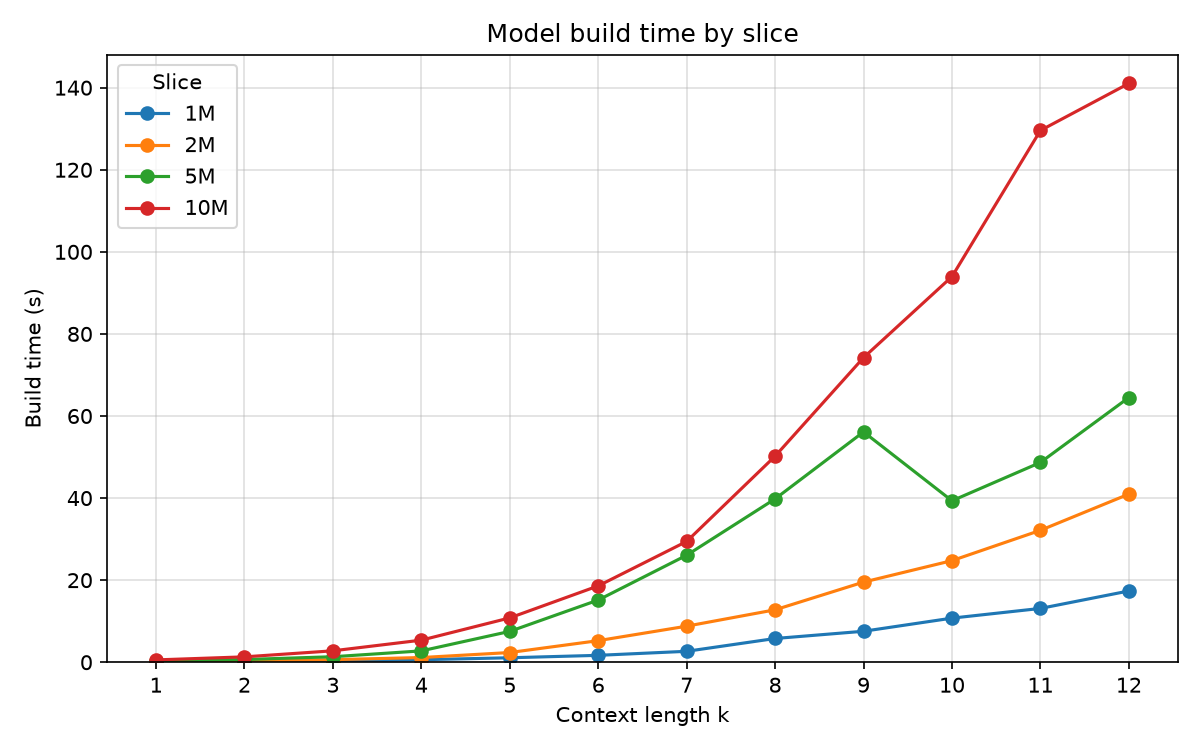
\includegraphics[width=\linewidth]{build_time_all.png}
    \caption{Tid til at bygge modellen.}
  \end{subfigure}
  \hfill
  \begin{subfigure}{0.49\textwidth}
    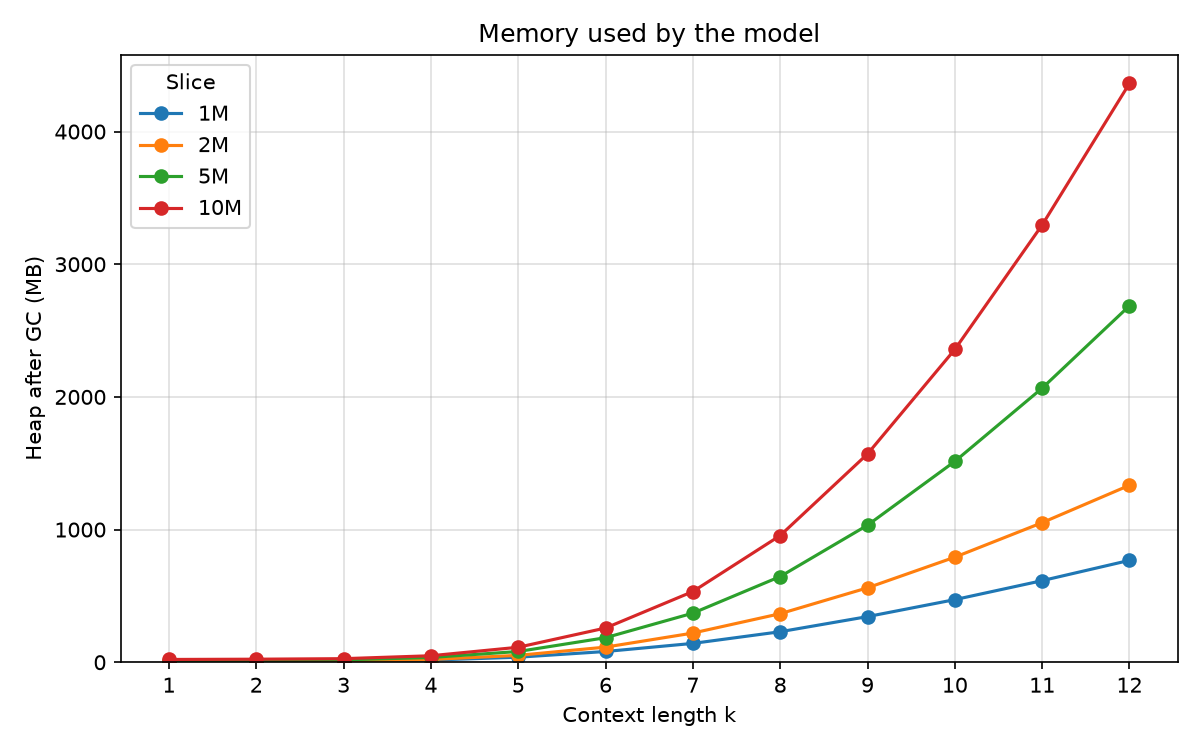
\includegraphics[width=\linewidth]{heap_all.png}
    \caption{Hukommelse brugt af modellen.}
  \end{subfigure}
  \caption{Byggetid og hukommelsesforbrug som funktion af kontekstlængden $k$ for
  de fire tekstudsnit.}
  \label{fig:resultater}
\end{figure}

\begin{table}[ht]
  \centering
  \begin{tabular}{lrrrr}
    \toprule
    Udsnit & $k$ & Kontekster & Byggetid & Hukommelse \\
    \midrule
    1M  & 3  & 15\,484      & 0{,}3 s   & 7 MB    \\
    1M  & 12 & 4\,560\,179  & 17 s      & 768 MB  \\
    10M & 3  & 33\,045      & 2{,}8 s   & 27 MB   \\
    10M & 12 & 25\,707\,907 & 141 s     & 4\,363 MB \\
    \bottomrule
  \end{tabular}
  \caption{Udvalgte målinger. Antallet af kontekster tæller alle længder fra 0 til $k$.}
  \label{tab:udvalg}
\end{table}

Figur~\ref{fig:resultater} og tabel~\ref{tab:udvalg} viser hovedresultaterne. For
små $k$ er modellen næsten gratis: der findes kun omkring 100 forskellige enkelttegn
og nogle få tusinde tegnpar, uanset hvor meget tekst vi træner på. Når $k$ vokser,
eksploderer antallet af forskellige kontekster, og både tid og hukommelse følger
med. På 10M-udsnittet går vi fra under ét sekund og 21 MB ved $k=1$ til over to
minutter og mere end 4 GB ved $k=12$. Kurverne ligger desuden i samme rækkefølge som
udsnittenes størrelse: dobbelt så meget tekst giver groft sagt en dobbelt så stor
model ved store $k$.

Der gemmer sig et interessant mønster i tallene. I teorien findes der $256^{12}$
mulige kontekster af længde 12, men modellen kan aldrig se flere, end der er
positioner i teksten. På 1M-udsnittet kommer der ved de høje værdier af $k$ omkring
0{,}9 millioner nye kontekster til, hver gang $k$ øges med én, altså næsten én ny
kontekst pr.\ tegn i teksten. Det betyder, at næsten hver eneste 12-tegnssekvens er
unik: den findes kun ét sted. Modellen er i praksis blevet en kopi af
træningsteksten, bare opdelt i overlappende stykker. Det er også derfor,
hukommelsen vokser lineært med tekstmængden.

Målingerne skal tages med et vist forbehold. De er lavet på en almindelig bærbar,
hvor andre programmer kørte samtidig, og samme kørsel ($1$M, $k=12$) tog f.eks.\
10{,}5 s i én omgang og 17 s i en anden, ligesom 5M-kurven har et tydeligt dyk ved
$k=10$. Den overordnede tendens er dog både tydelig og stabil.

\section{Hvad modellen skriver}

Tallene fortæller kun halvdelen af historien; det mest lærerige var at læse den
tekst, modellen selv producerer. Her er korte uddrag fra modeller bygget på
1M-udsnittet:

\begin{description}
  \item[$k=1$:] \textit{ve tu wis he r s t thist Asikithe ku cknshavek warst f end owointea}
  \item[$k=3$:] \textit{Corpheus wouldn't him the side fore and lovelowing in tely cond, who he reall head loor}
  \item[$k=5$:] \textit{Bo-Katan is though the put on something of one in front. 'Well asks. Charon's been a hand.}
  \item[$k=8$:] \textit{He turned and glanced up at that those look like the road as a wonderful and lively complexion}
  \item[$k=12$:] \textit{After that time the buns were all eaten, the prizes were all loaded up, and it seemed everyone else is gonna be a good day.}
\end{description}

Udviklingen er tydelig. Med $k=1$ kender modellen kun bogstavfrekvenser og typiske
bogstavpar, så resultatet ligner engelsk på afstand, men indeholder næsten ingen
rigtige ord. Ved $k=3$ falder korte, almindelige ord på plads, mens de længere ord
bliver til fantasiord som \textit{lovelowing}. Ved $k=5$ er næsten alle ord rigtige,
men sætningerne giver ikke mening. Ved $k=8$ dukker korte grammatiske stumper op, og
ved $k=12$ læses teksten næsten som rigtig prosa.

Men den flotte tekst ved $k=12$ er i en vis forstand snyd. Fordi næsten hver
12-tegnskontekst kun findes ét sted i teksten, er der ofte kun ét muligt næste tegn,
og modellen kopierer derfor lange passager ordret. Den skifter kun spor, når to
steder i teksten tilfældigvis deler de samme 12 tegn. Modellen \emph{husker} altså mere,
end den \emph{generaliserer}.

\section{Hvad vi har lært}

Opgaven har givet os en konkret fornemmelse af et grundlæggende dilemma i
sprogmodellering. En kort kontekst giver en model, der generaliserer, fordi hver
kontekst er set mange gange, men den har ingen hukommelse og skriver volapyk. En
lang kontekst giver flot tekst, men kun fordi modellen genbruger det, den har set,
og den kræver enorme mængder hukommelse. Der findes ikke noget $k$, der både er
lille nok til at generalisere og stort nok til at fange betydningen af en hel
sætning.

Problemet er, at en tælletabel behandler hver kontekst som helt uafhængig af alle
andre. \textit{``the cat sat''} og \textit{``the dog sat''} har intet til fælles for
vores model, selvom de for et menneske er næsten ens. Det er præcis her, moderne
sprogmodeller adskiller sig: i stedet for at slå op i en tabel bruger de neurale
netværk, der repræsenterer ord og sammenhænge som tal, sådan at lignende kontekster
får lignende repræsentationer. Det gør det muligt at se tusindvis af tokens tilbage,
uden at tabellen eksploderer, og at sige noget fornuftigt om en sætning, modellen
aldrig har set før. Samtidig minder vores resultat ved $k=12$ om en kendt bekymring
ved store modeller, nemlig at de kan komme til at gengive deres træningsdata ordret.

Vi har også lært noget mere praktisk: valget af datastruktur kan være forskellen på
et program, der virker, og et, der går ned. Den samme matematiske model fyldte ti
gange mindre, alene fordi vi lod være med at gemme alle nullerne. Og vi har set, at
måling af tid og hukommelse kræver omtanke, f.eks.\ at man bør rydde op i
hukommelsen, før man måler, og tage enkeltmålinger med et gran salt.

\section{Konklusion}

Vi har bygget og målt en simpel tegnbaseret sprogmodel for kontekstlængder fra 1 til
12 på tekstudsnit fra 1 til 10 millioner tegn. Efter at have rettet modellens
hukommelsesproblem med en sparsom repræsentation kunne vi vise, at antallet af
kontekster, byggetiden og hukommelsesforbruget vokser kraftigt med $k$ og omtrent
lineært med tekstmængden. Teksten bliver mere realistisk, jo større $k$ er, men ved
de høje værdier skyldes det, at modellen kopierer træningsteksten frem for at forstå
den. Den vigtigste indsigt for os er derfor, at det ikke er nok at huske mere
kontekst; man har brug for en model, der kan generalisere \emph{mellem} kontekster,
og det er netop det, moderne sprogmodeller er bygget til.

\end{document}
